\begin{savequote}[8cm]
Far out in the uncharted backwaters of the unfashionable end of the western spiral arm of the Galaxy lies a small unregarded yellow sun. Orbiting this at a distance of roughly ninety-two million miles is an utterly insignificant little blue green planet whose ape-descended life forms are so amazingly primitive that they still think digital watches are a pretty neat idea.
  \qauthor{--- D. Adams, The Hitchhiker's Guide to the Galaxy}
\end{savequote}

\chapter{Introduction}\label{ch:1-intro}

\minitoc

How do you design and assemble something on the nanoscale? Imagine building something with lego bricks; you choose the building blocks you want and use your hands to attach them where you want them to be. However, for nanoscale objects, it is difficult to have that level of control. Instead, more success has been had by imitating nature and letting the building blocks assemble themselves. This thesis will cover novel methods and tools to design such self-assembling nanostructures.

\section{Thesis structure}
This thesis covers two related projects, both concerning the design and modular self-assembly of nanostructures. Each project is introduced by a separate chapter on its relevant history and background.

The first project, introduced by Chapter \ref{ch:polycubes_intro}, covers an abstract self-assembly model called \emph{polycubes}. Chapter \ref{ch:polycubes1} details the model and the shapes that assemble when randomly sampling the input space. Chapter \ref{ch:polycubes2} presents the results on the reverse problem; given a polycube shape, what input rules will assemble it and can you minimise input complexity?

The second project takes a more detailed view of self-assembly design. Chapter \ref{ch:oxview_intro} gives a background on computer-aided design tools for nucleic acid structures, followed by an introduction of the models used to simulate such designs. Chapter \ref{ch:oxview} then presents my contributions to \emph{oxView}, a web-based tool for the visualisation, design, and integration of DNA, RNA and protein structures.

This chapter serves as an introduction to both projects, providing background on DNA and RNA self-assembly.

%\section{Scope of the thesis}


\section{DNA design}
Deoxyribonucleic acid (DNA) is a string-like molecule used to encode the genes of living systems \cite{calladine1997understanding}. These strings are made up of units called \emph{nucleotides}, consisting of a sugar-phosphate backbone as well as one of four possible bases: \emph{adenine} (A), \emph{thymine} (T) \emph{cytosine} (C), and \emph{guanine} (G).

Through Watson-Crick base-pairing, A forms two hydrogen bonds with T, while G forms three with C, making DNA double-stranded. Each strand has a directionality, conventionally represented as going from the 3' to the 5' end of the strand, making the duplex anti-parallel.

The bases of the duplex are hydrophobic, while the sugar-phosphate backbone is hydrophilic, which means that the bases ``hide'' on the inside of the duplex to avoid contact with water molecules. However, the backbone distance is about 6 Å (0.6 nm), while the bases would need to be at a distance of 3.3 Å (the thickness of the base) to not leave any room for water \cite{calladine1997understanding}. To solve this, the DNA duplex forms a double helix structure with a radius of about 9 Å, placing everything at an energetically comfortable distance.

While a single double-helix is the most natural confirmation, it is possible for strands to branch into multiple junctions. For example, the Holliday junction is a junction between four double-helical arms, shown in Figure \ref{fig:holliday} in one of its possible configurations.

\begin{figure}
    \centering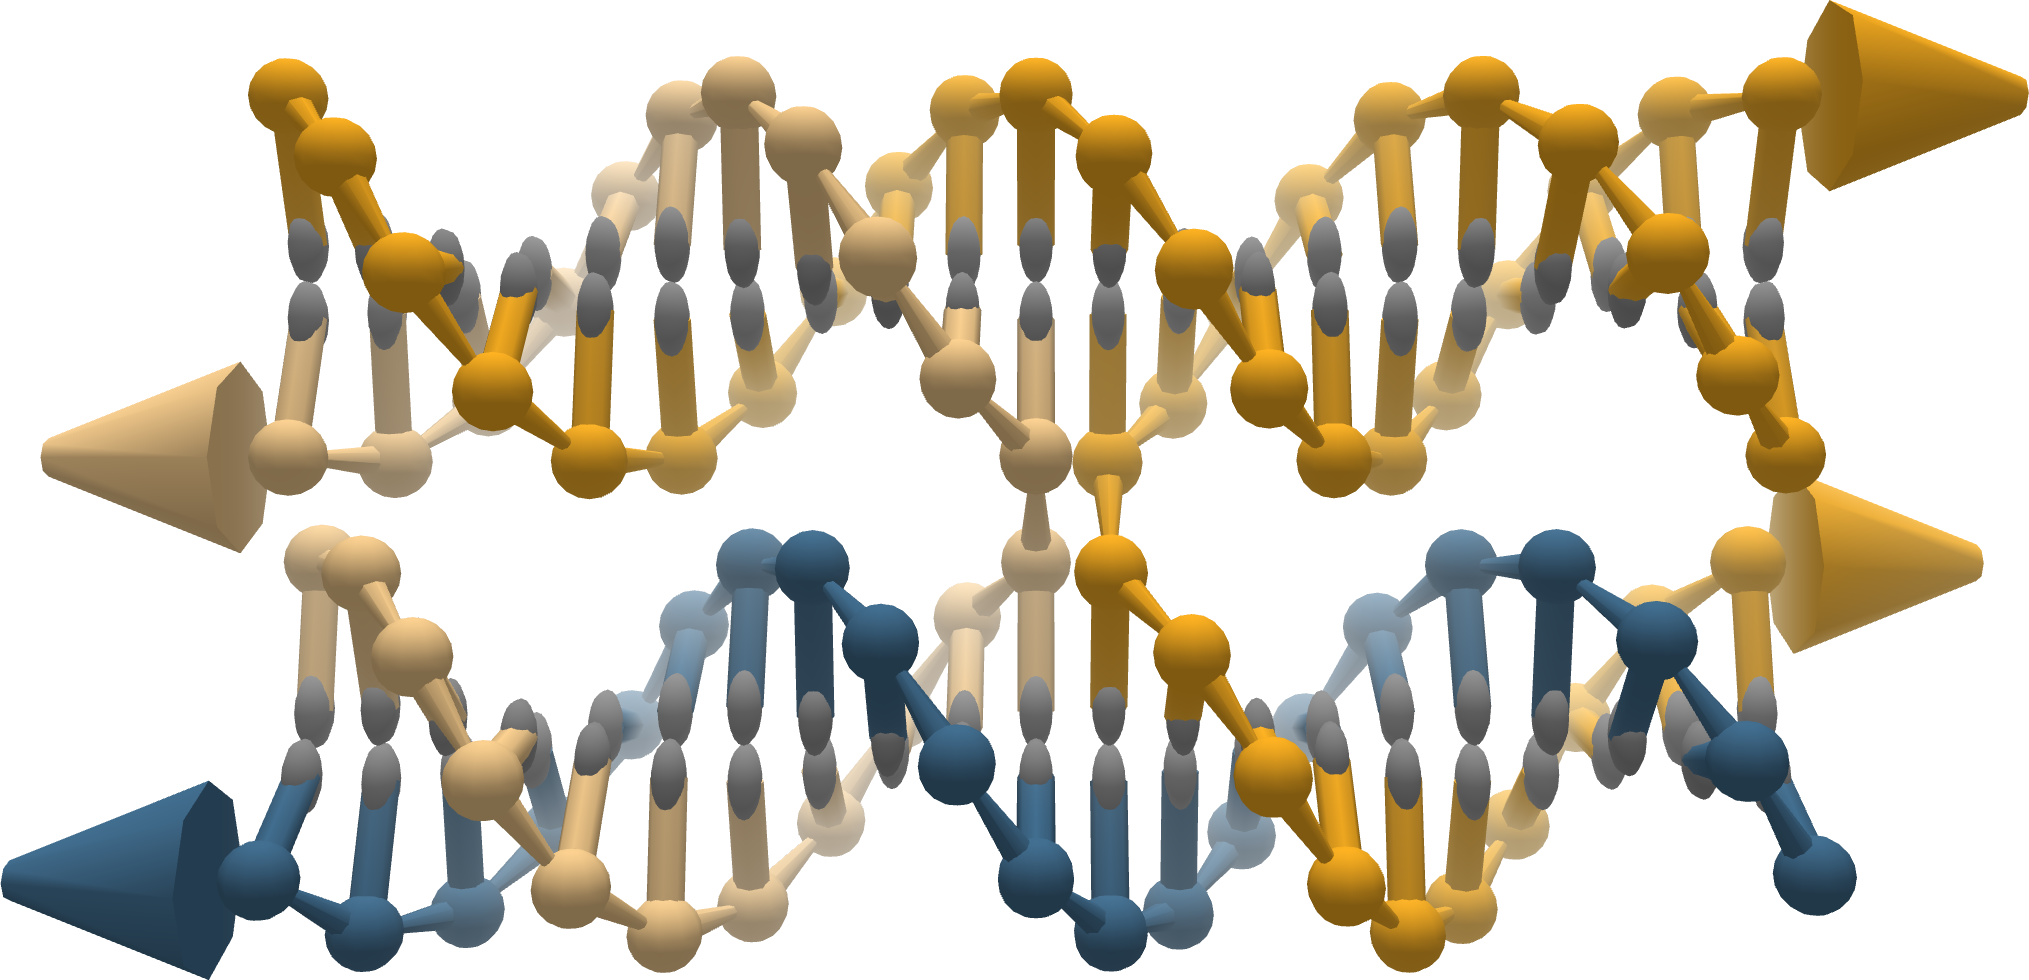
\includegraphics[width=\textwidth]{figures/holliday.png}
    \caption{Holliday junction, designed in oxView. Cones at the end indicates the 3' end of each of the four strands.}
    \label{fig:holliday}
\end{figure}

%https://www.rcsb.org/structure/1M6G

%Double-stranded DNA has a persistence length of approximately [], while single-stranded sections are much more flexible,

By designing sequences with complementary domains for the intended duplex regions, it is possible to create many different DNA motifs and structures \cite{seeman_2016}.

%% Add more here

A breakthrough in the field of structural DNA nanotechnology was the DNA origami technique \cite{rothemund2006folding} a now popular and proven method for creating larger irregular structures using DNA. The principle behind it, as illustrated in Figure \ref{fig:dnaOrigami}, is to use short staple strands to fold one long viral scaffold strand into the desired structure.

\begin{figure}
    \centering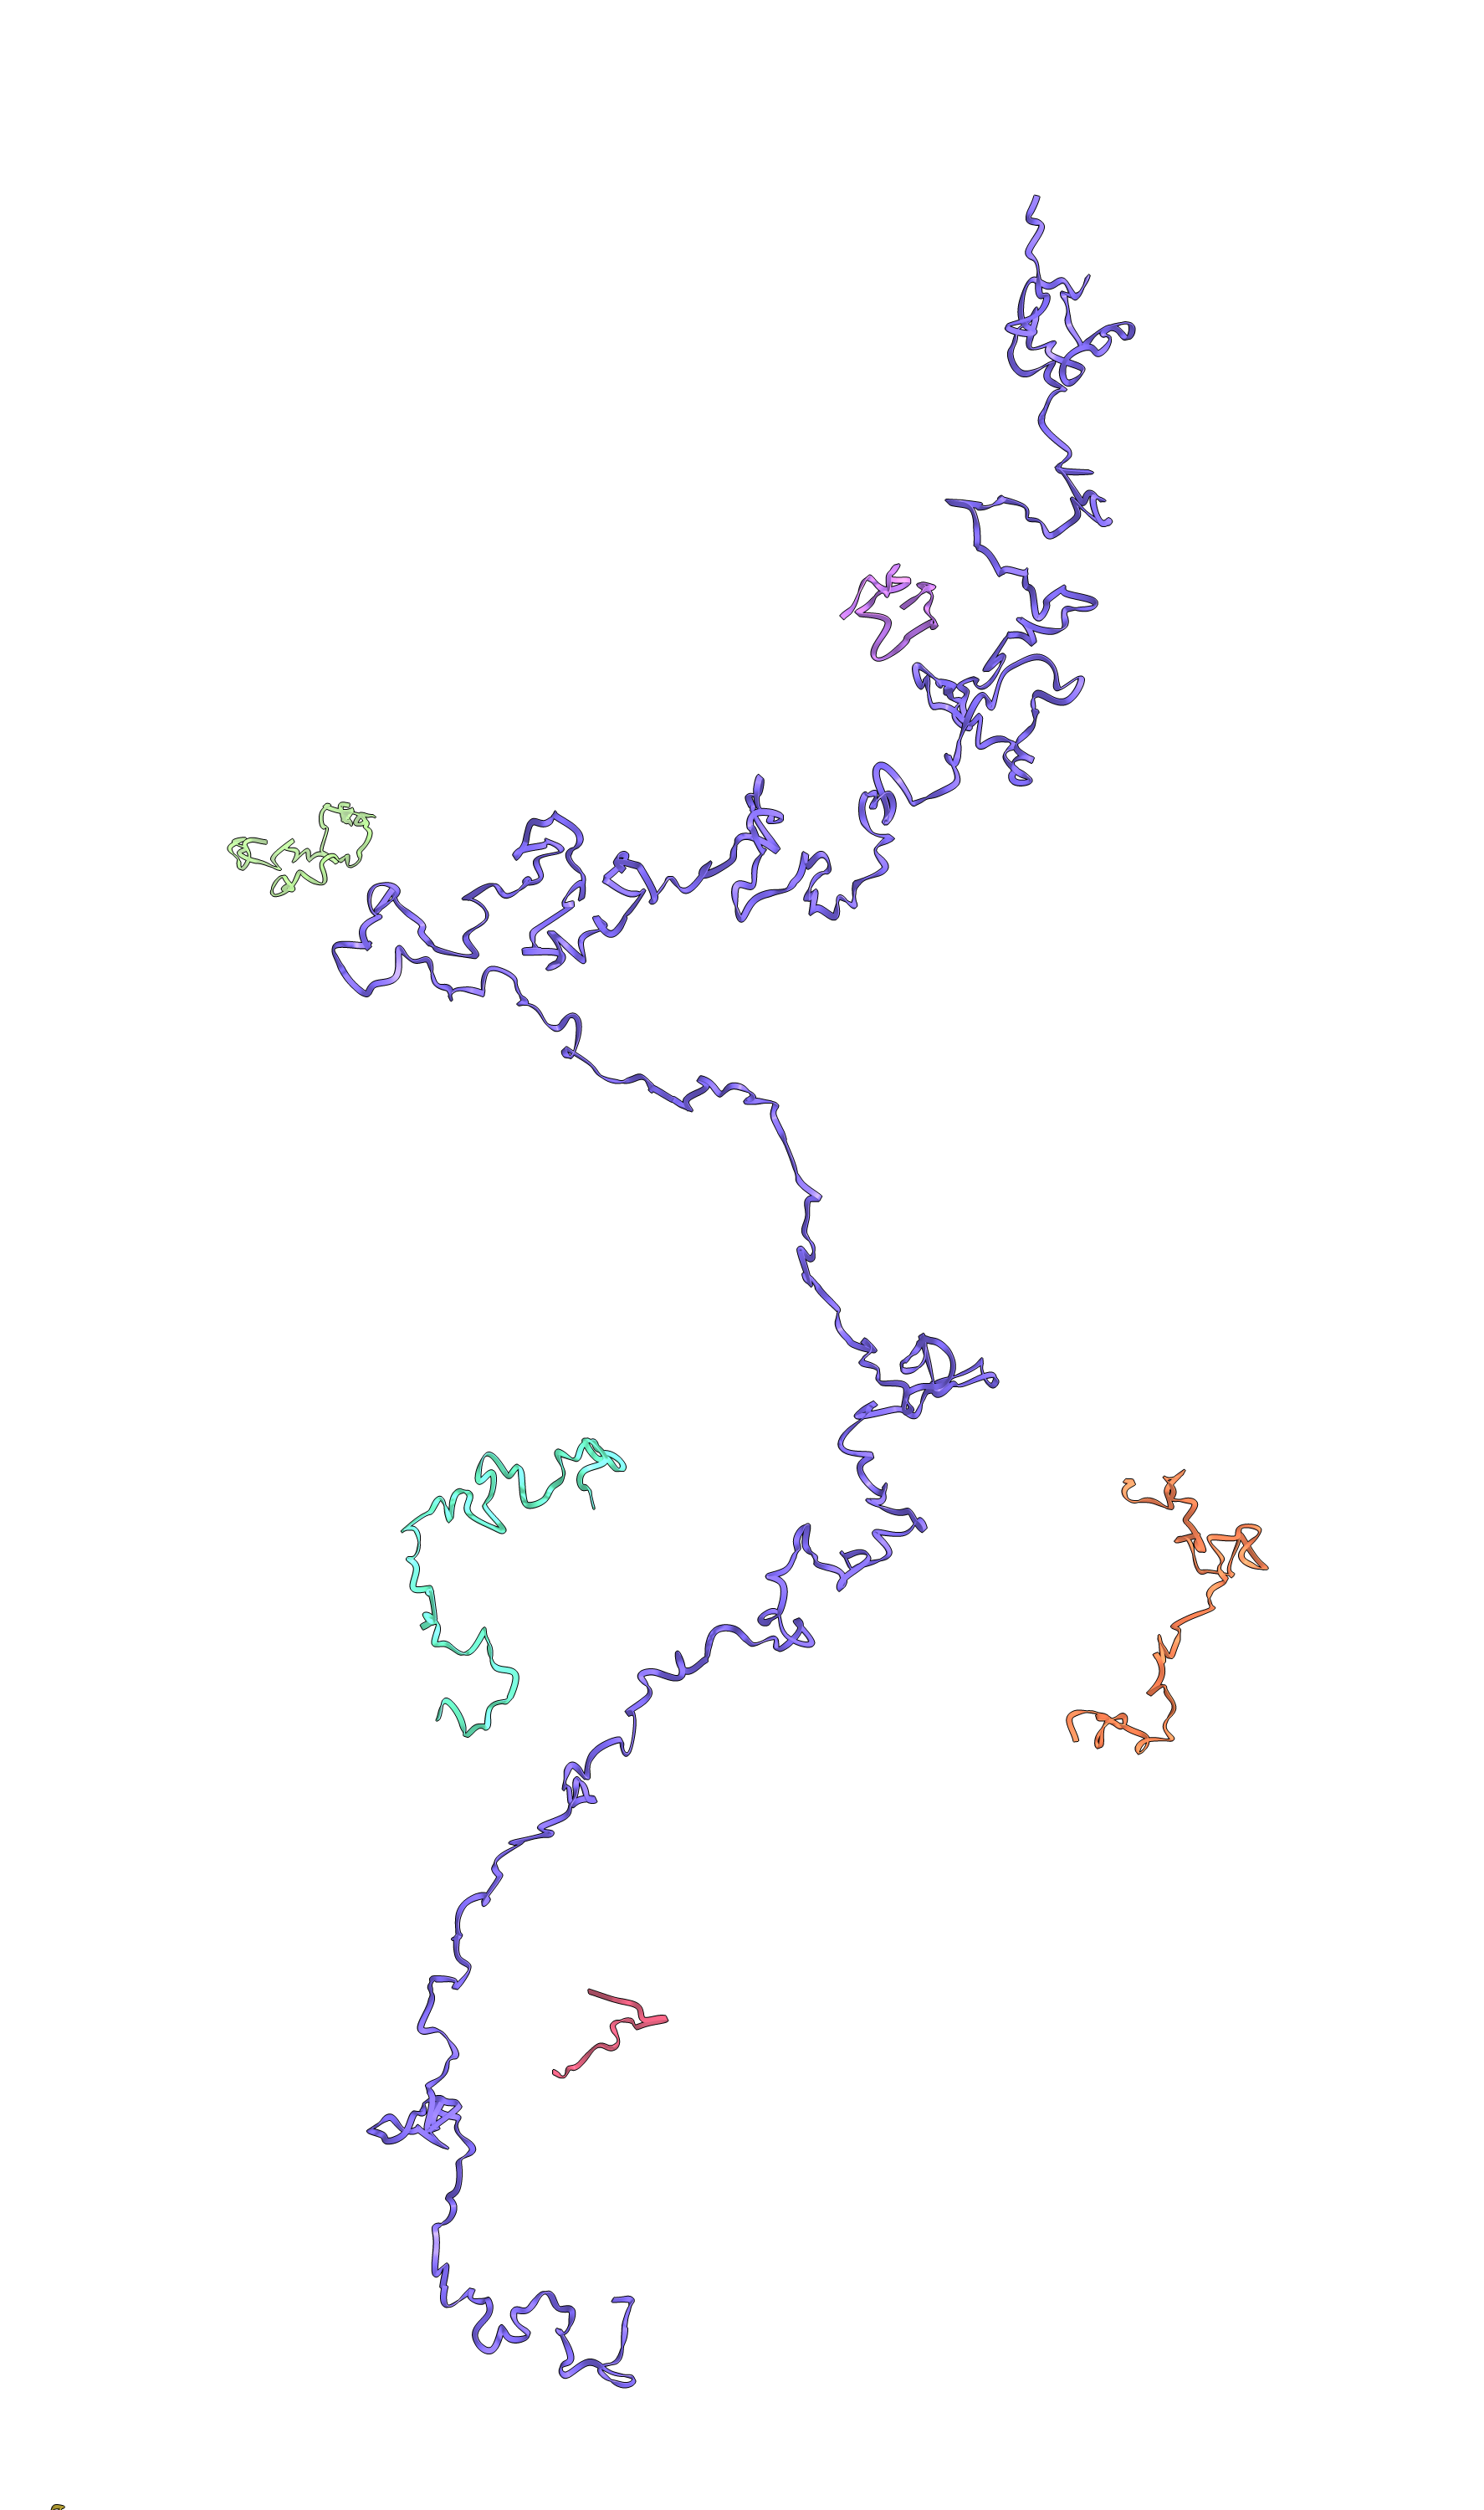
\includegraphics[width=\textwidth/5]{figures/melt/melted.png}\hfill
%    \centering\includegraphics[width=\textwidth/5]{figures/melt/intermediate2.png}\hfill
    \centering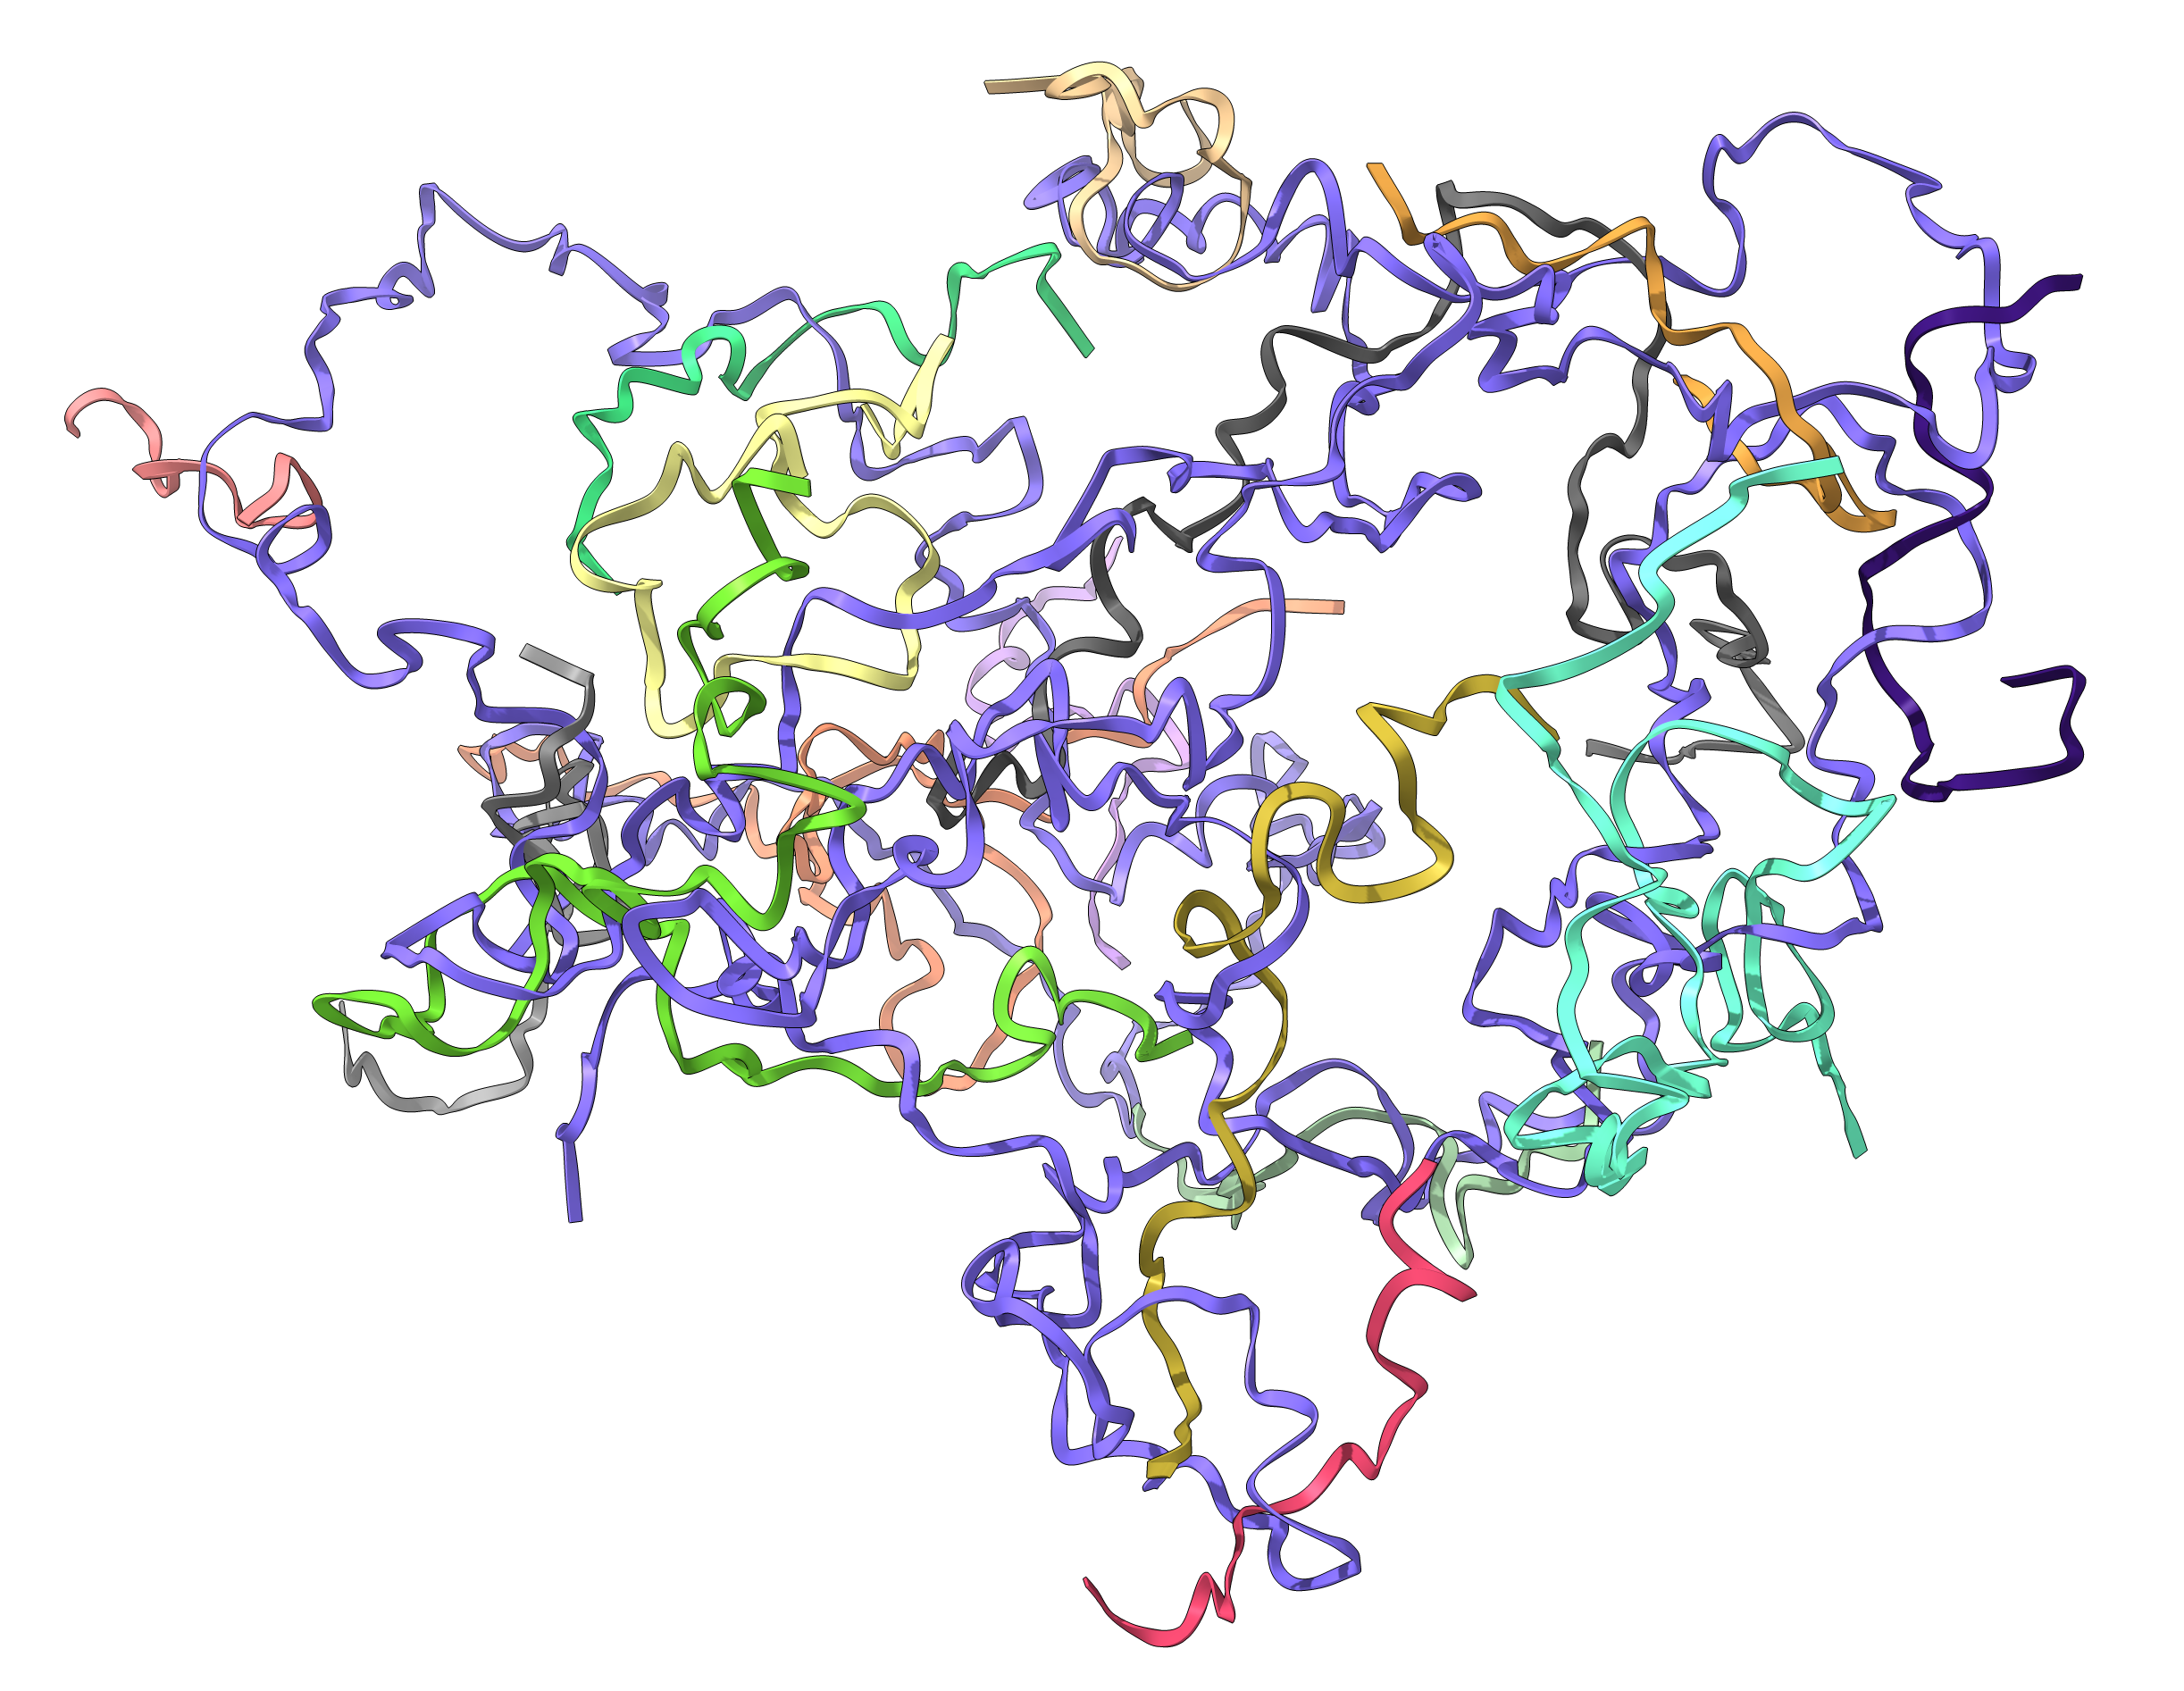
\includegraphics[width=\textwidth/3]{figures/melt/intermediate1.png}\hfill
    \centering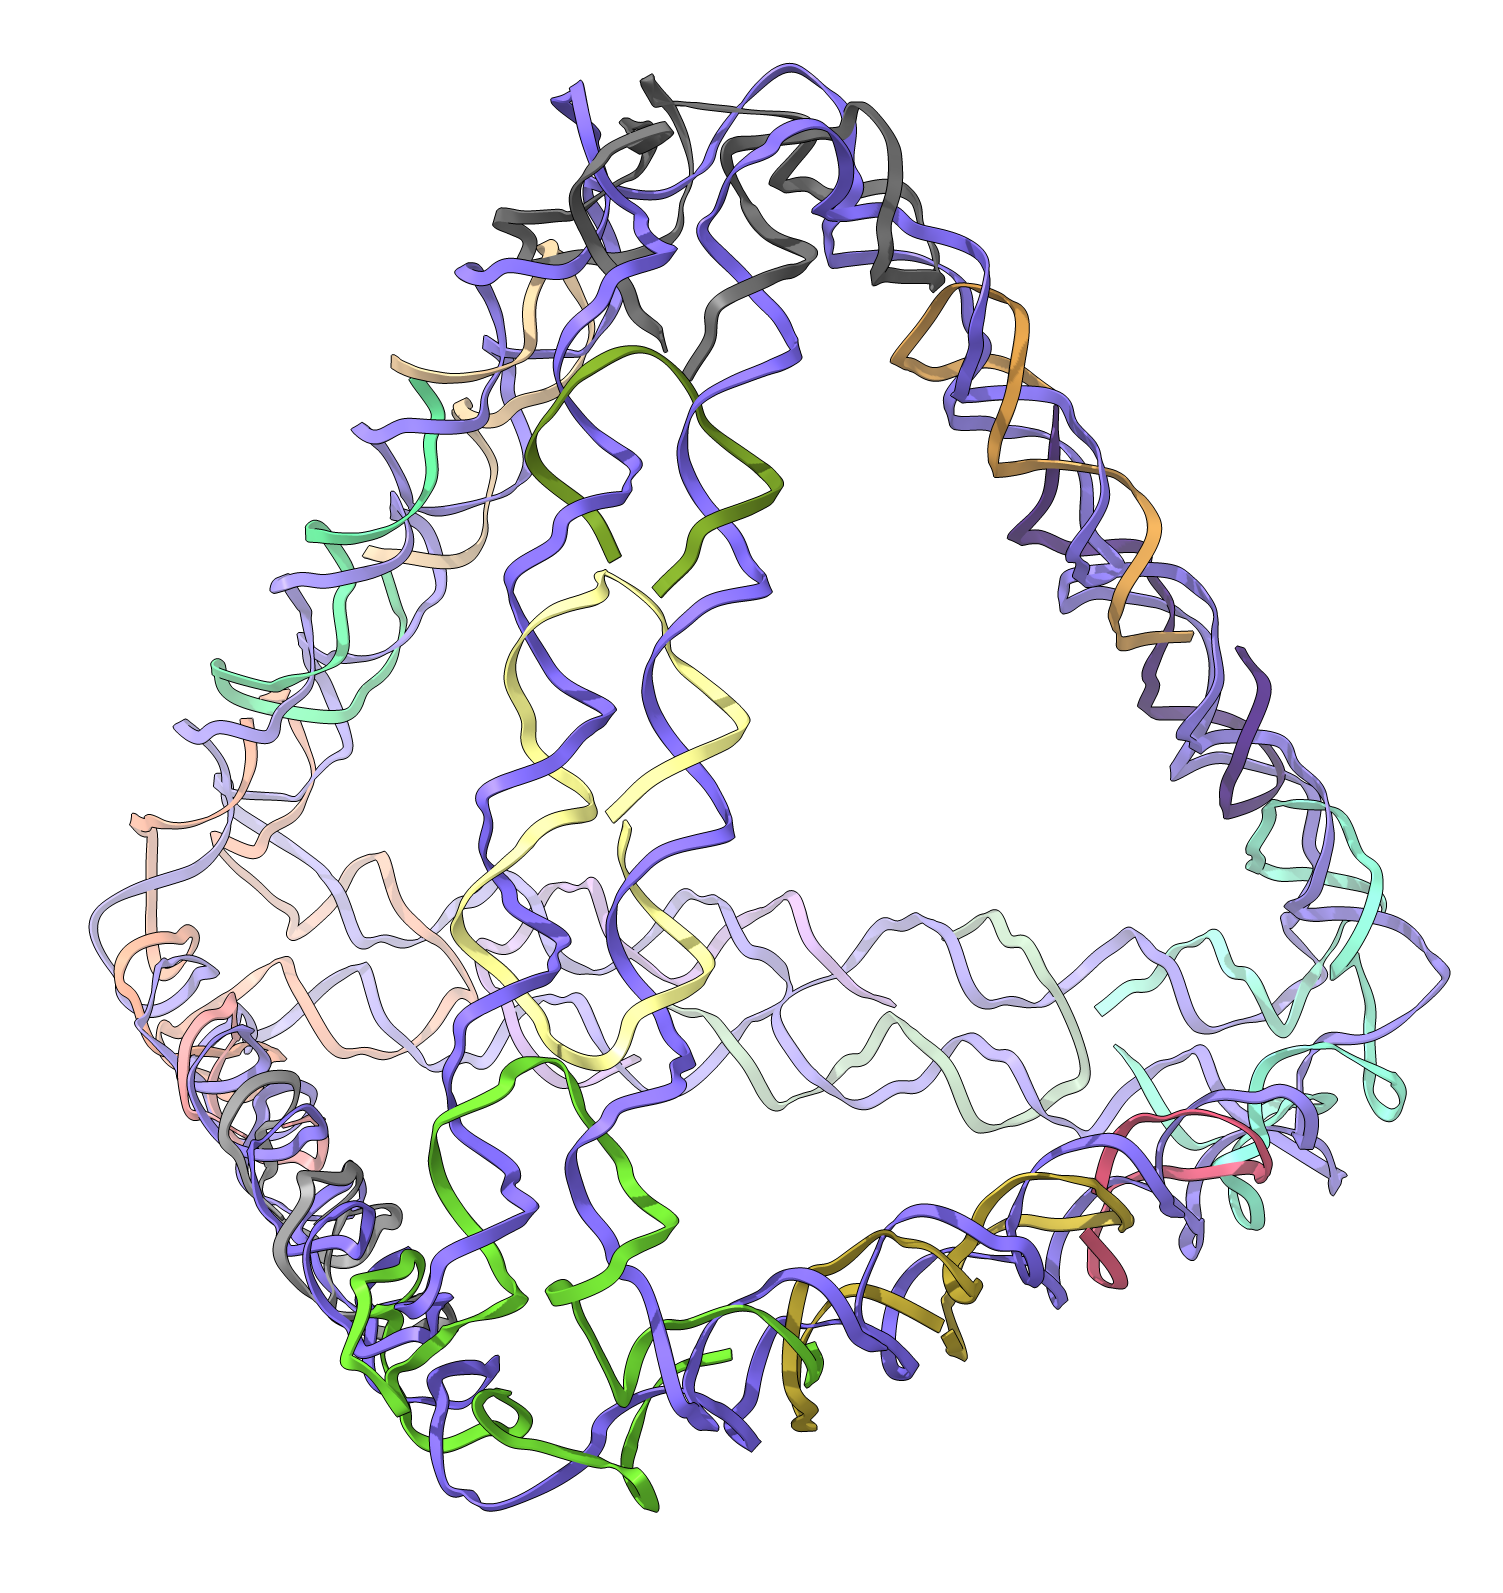
\includegraphics[width=\textwidth/3]{figures/melt/assembled.png}
    \caption{Illustration of DNA origami self-assembly of a tetrahedron. A long scaffold strand (purple), obtained from a virus, is folded into the desired shape by multiple short staple strands binding to complementary domains of the scaffold. Tetrahedron design obtained from \url{https://cando-dna-origami.org/examples/} and melted using oxDNA simulation \cite{ouldridge2010dna}.
    }
    \label{fig:dnaOrigami}
\end{figure}

Using design tools such as caDNAno \cite{cadnano}, it has become relatively easy to design structures of any given form. See Section \ref{sec:design_tools} for an introduction to additional such tools. However, the size of the origami is limited by the length of the scaffold. This motivates researchers to investigate modular approaches, some of which will be described in Section \ref{sec:experimental_appl}.

\section{RNA design}
\label{sec:RNA_design}
Ribonucleic acid (RNA) is very similar to DNA, but with the \emph{thymine} base replaced by \emph{uracil} (U). Just like DNA, it is possible to use it as a self-assembling building material.

Biologically, DNA is transcribed into RNA by the RNA polymerase enzyme as part of gene expression. While DNA folding is easier to predict, the fact that RNA is more reactive than DNA also offers the possibility of a more useful structure; for example, by incorporating aptamers, enzymes and other such functionalities \cite{guo2010emerging}.

Geary et al., from the Andersen lab in Aarhus, demonstrated a method \cite{geary2014single, sparvath2017computer, geary2021rna} for co-transcriptionally folded RNA origami in 2014, which also enables folding \emph{in vivo}. The design used a set of tertiary RNA motifs, such as kissing hairpins and double crossovers, to fold the transcribed RNA strand into the desired structure. The Andersen lab is one of the network partners, and I have spent a two-month secondment there working with their RNA origami method.

\begin{figure}[h]
    \centering
    \begin{overpic}[width=\textwidth]{figures/rna_origami.png}
        \put(0,600){a)}
        \put(0,250){b)}
        \put(0,110){c)}
        \put(510,600){d)}
        \put(510,430){e)}
        \put(510,310){f)}
        \put(510,150){g)}
    \end{overpic}
    \caption{Co-transcriptional folding of RNA origami, adapted from \cite{geary2021rna}. a) The set of RNA motifs used as modular building blocks. b) Schematic of the modules connected to form a single strand. c) Atomistic model of the design in b). d) Shows the text-based blueprint used to create designs, while e), f), and g) shows scripts developed to aid the visualisation and preform sequence design for the origami.}
    \label{fig:rna_origami}
\end{figure}

% "The emerging field of RNA nanotechnology121 might seem more promising in this regard because RNA is readily transcribed into a single strand in cells, which can be directly folded into a programmed nanostructure"
% https://www.nature.com/articles/nnano.2011.187

\section{Algorithmic Information Theory and input-output maps}
\label{sec:AIT}
% https://www.ox.ac.uk/news/science-blog/%E2%80%98simplicity-bias%E2%80%99-science

% https://www.nature.com/articles/s41467-018-03101-6

% https://solo.bodleian.ox.ac.uk/permalink/f/89vilt/oxfaleph022417805

%Some things, whether in the form of a shape, a song, or a binary string, require less information to describe than others.

If you have a monkey pressing random keys on a typewriter, you would expect it to produce every string of length \(N\) with equal probability (assuming the keystrokes were indeed truly random). With \(k\) keys on the keyboard, the probability for any string of length \(N\) is then \(k^{-N}\). For example, the title of this thesis, while unlikely to appear randomly, would be equally as probable as any other 50-character string, see the three example strings below:
\begin{lstlisting}[numbers=left]
  DESIGN AND MODULAR SELF-ASSEMBLY OF NANOSTRUCTURES
  SHWDRVWKFORWJDOEXOZLSBNREKC Z  VSDJJF  ROKFYRVMIUI
  AAAAAAAAAAAAAAAAAAAAAAAAAAAAAAAAAAAAAAAAAAAAAAAAAA
\end{lstlisting}

However, some strings can have a description shorter than a full listing of the letters it contains. For example, string number three above could be described simply as ``Print \texttt{A}, 50 times'', or if we use the C programming language:

\begin{lstlisting}[language=c]
for(int i=50; i--;) printf("A");
\end{lstlisting}

There are also a number of possible valid variations of the code above, with different variable names and coding conventions, all producing the same output. In other words, not only is the description shorter than writing out the full string but multiple inputs map to the same output, increasing the probability of the output further.

The concept of using the shortest possible computer program that can describe an object (for example, a binary string) to determine its complexity is central within the field of Algorithmic Information Theory (AIT) and is called Kolmogorov complexity (or Solomonoff–Kolmogorov–Chaitin to give full credit) \cite{LiMing2019AitK}. More specifically, the Kolmogorov complexity \(K(x)\) of an output \(x\) is the length of the shortest program that generates \(x\) on a Universal Turing Machine (UTM).

AIT includes the \emph{coding theorem}, introducing lower and upper bounds for the probability \(P(x)\) of generating a binary string \(x\) as \(2^{-K(x)} \le P(x) \le 2^{-K(x) + \mathcal{O} (1)}\). In other words, low-complexity outputs are exponentially more likely to generated by random input compared to high-complexity outputs. This could be compared to how, intuitively, there are likely more programs generating the ``simple'' string number 3 above compared to the randomly generated number 2.

However, finding the shortest program for an output is far from trivial (in general, it is in fact \emph{uncomputable}, due to the \emph{halting problem}). Fortunately, Dingle at al \cite{dingle2018input} were able to derive an upper bound to the probability using a computable approximation \(\widetilde{K}(x)\) of the Komologrov complexity:

\[
  P(x) \lesssim 2^{-a\widetilde{K}(x) -b}
\]

where \(a\) and \(b\) are constants that depend on the input-output map used (but are independent of \(x\)).


